% !TeX spellcheck = en_US
\documentclass[french]{yLectureNote}

\title{Électrocinétique}
\subtitle{Physique}
\author{Paulhenry Saux}
\date{\today}
\yLanguage{Français}

\professor{Allard}%allard@irsamc.ups-tlse.fr
\usepackage{graphicx}%----pour mettre des images
\usepackage[utf8]{inputenc}%---encodage
\usepackage{geometry}%---pour modifier les tailles et mettre a4paper
%\usepackage{awesomebox}%---pour les boites d'exercices, de pbq et de croquis ---d\'esactiv\'e pour les TP de PC
\usepackage{tikz}%---pour deiffner + d\'ependance de chemfig
\usepackage{tkz-tab}
\usepackage{chemfig}%---pour deiffner formules chimiques
\usepackage{chemformula}%---pour les formules chimiques en \'equation : \ch{...}
\usepackage{tabularx}%---pour dimensionner automatiquement les tableaux avec variable X
\usepackage{awesomebox}%---Pour les boites info, danger et autres
\usepackage{menukeys}%---Pour deiffner les touches de Calculatrice
\usepackage{fancyhdr}%---pour les en-t\^ete personnalis\'ees
\usepackage{blindtext}%---pour les liens
\usepackage{hyperref}%---pour les liens (\`a mettre en dernier)
\usepackage{caption}%---pour la francisation de la l\'egende table vers Tableau
\usepackage{pifont}
\usepackage{array}%---pour les tableaux
\usepackage{lipsum}
\usepackage{yFlatTable}
\usepackage{multicol}
\newcommand{\Lim}[1]{\lim\limits_{\substack{#1}}\:}
\renewcommand{\vec}{\overrightarrow}
\begin{document}
\setcounter{chapter}{2}
	\chapter{Théorèmes généraux de l'électrocinétique}
\section{Principe de superposition}
%TODO
% \begin{theorem}[Théorème de Milmann]
%
% \end{theorem}
% On doit connaitre les potentiels des autres points par référence par rapport au point $B$.
\begin{theorem}[Principe de superposition]
 Dans un circuit linéaire, le courant crée dans une branche donnée par plusieurs sources indépendantes agissant simultanément est égal à la somme algébrique des courants produits dans cette m\^eme branche par toutes les sources agissant séparément.
\end{theorem}
La démonstration repose sur la linéarité des équations.\marginTips{C'est valable pour les générateurs de tension et de courant, donc pour la tension et le courant.}
\checkInfo{En pratique}{En pratique, pour calculer la contribution d'une source, on va passiver les autres. On passive un générateur de tension idéal en le remplaçant par un intérupteur fermé. On passive un générateur de courant en le remplaçant par un interrupteur ouvert.}
\subsection{Exemple 1}
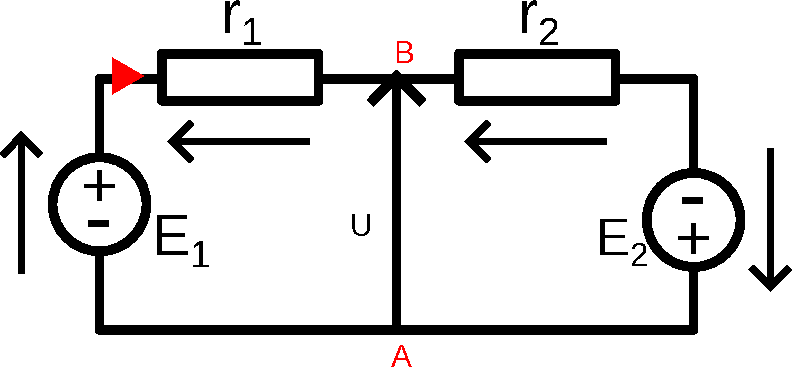
\includegraphics[scale=0.5]{c3-1}
\subsubsection{Avec la loi des mailles}

On applique la loi des mailles sur la maille la plus grande : $E_1-U_{r1}-U_{r2} + E_2 = 0$ et sur celle de gauche : $E_1-U_{r_1} - U = 0$. On cherche $U$.

Par l'équation 1 :$E_1+E_2=(R_1+R_2)i\Rightarrow i = \frac{E_1+E_2}{R_1+R_2}$.

On injecte l'expression de $i$ dans la deuxième équation pour trouver $U$ : $U = E_1-R_1(\frac{E_1+E_2}{R_1+R_2}) = \frac{R_2E_2-R_1E_2}{R_1+R_2}$

\subsection{Principe de superposition}

$U = U^{(1)} + U^{(2)}$ c'est à dire la tension avec seulement $E_1$ et seulement $E_2$.

On passive le générateur $E_2$ pour obtenir $ U^{(1)}$.

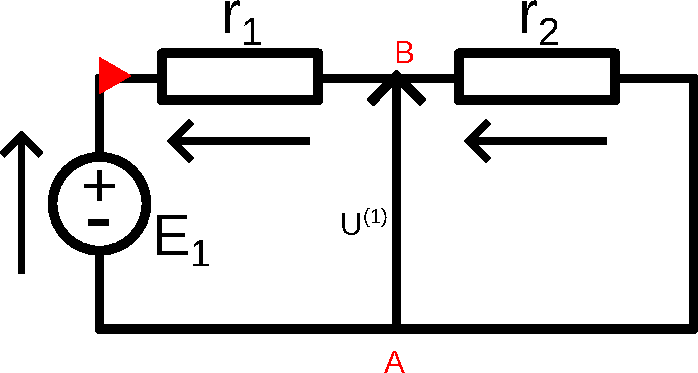
\includegraphics[scale=0.5]{c3-2}

On remarque que $U^{(1)} = U_{R_2}$ et en appliquant la formule du pont diviseur de tension : $U^{(1)} = E_1\frac{R_2}{R_1+R_2}$

On passive le générateur $E_1$ pour obtenir $ U^{(2)}$.

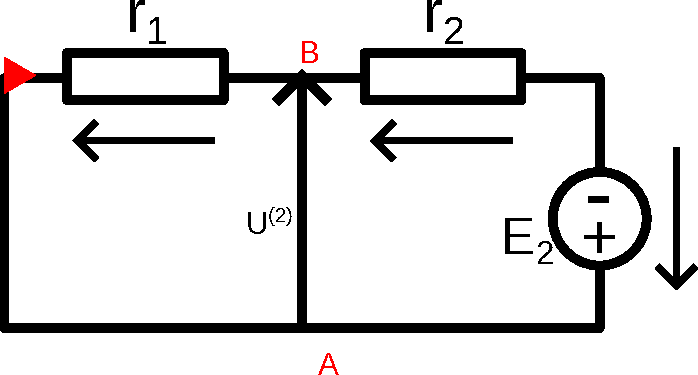
\includegraphics[scale=0.5]{c3-3}

On remarque que $U^{(2)} = -U_{R_1}$ et en appliquant la formule du pont diviseur de tension : $U^{(2)} =- E_2\frac{R_1}{R_1+R_2}$.

\subsection{Exemple 2}
Le but est de trouver la tension $U$.

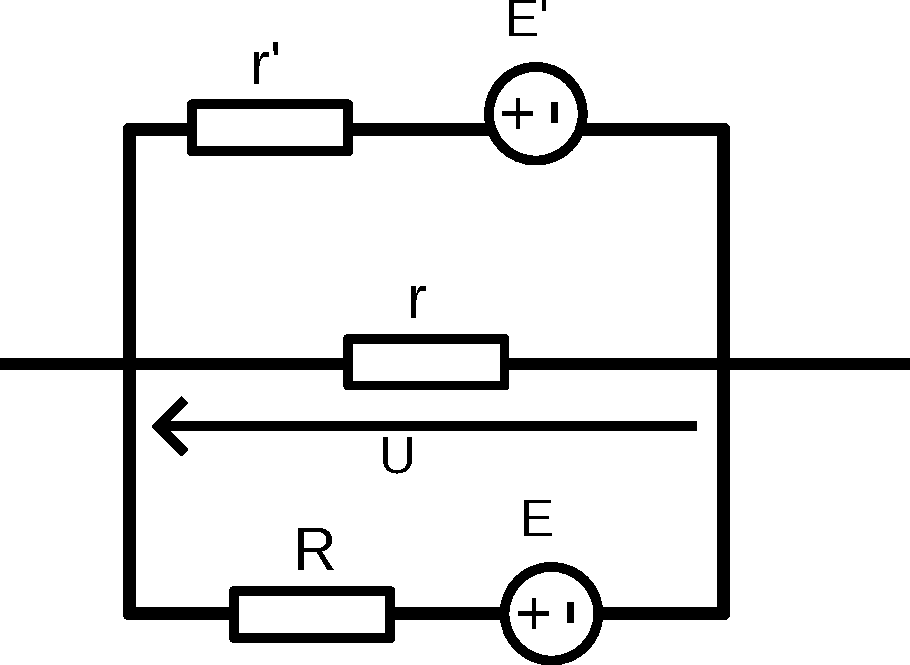
\includegraphics[scale=0.3]{c3-4}

On cherche $U^{(1)}$ en passivant $E'$. On introduit aussi une résistance équivalente : $r'//r = \frac{rR'}{R'+r}$. On reconnait aussi un pont diviseur de tension entre $R$ et la résistance équivalente : $U^{(1)} = U_{r'//r} = E\frac{r'//r}{R+r'//r}= E\frac{rR'}{R'r+rR+RR'}$.

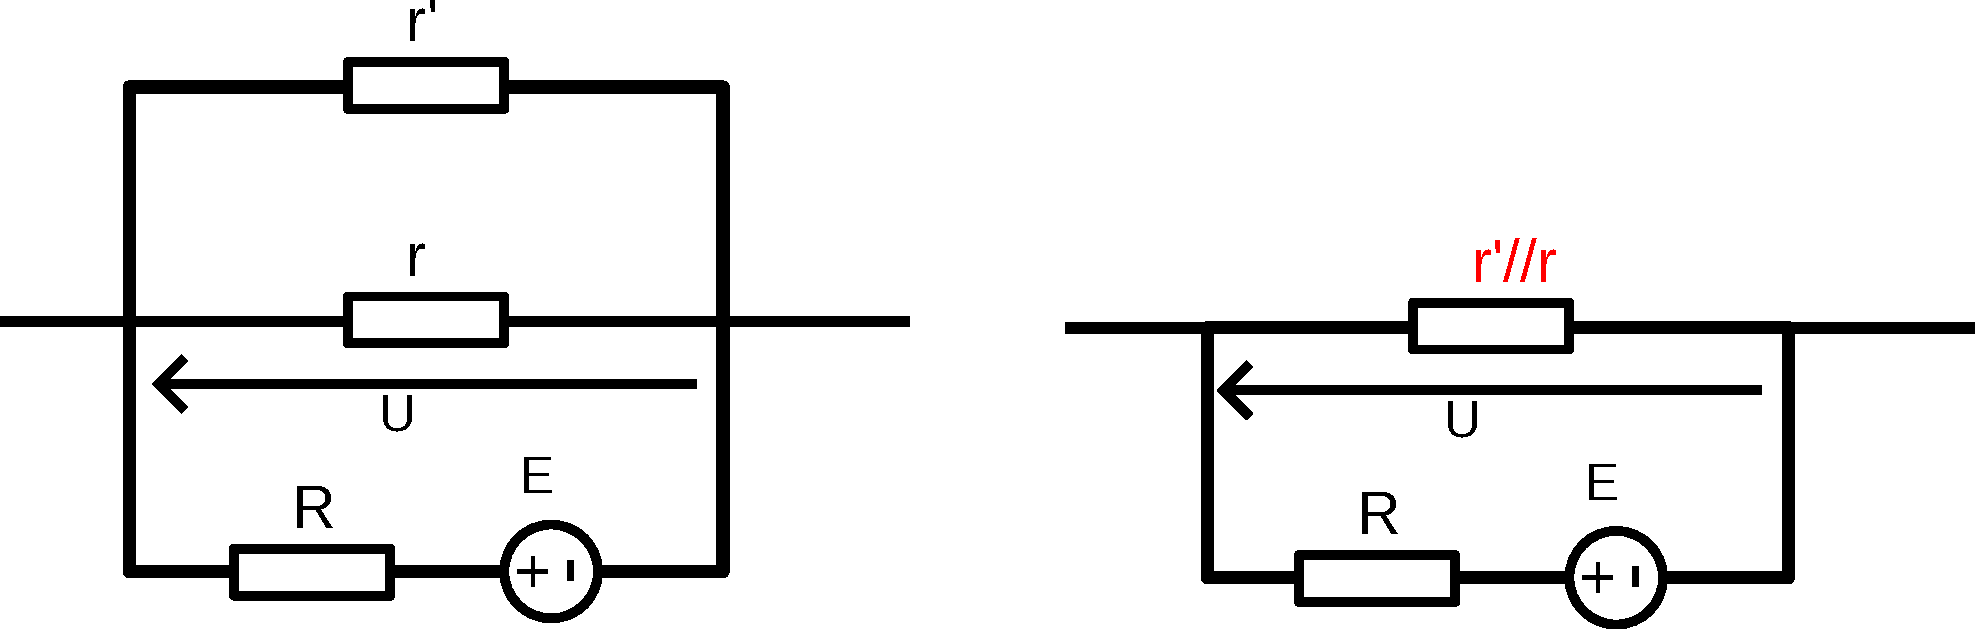
\includegraphics[scale=0.3]{c3-5}

On cherche $U^{(2)}$ donc on passive $E$ de la m\^eme manière. On obtient $U^{(2)} = E'\frac{rR}{R'r+rR+RR'}$.

La réponse est la somme des 2 tensions : $U = \frac{ErR'+E'rR}{R'r+rR+R'R}$.
\section{Théorème de Thévenin}
On suppose que $D$ est un dip\^ole et il ne contient aucune source liée à une grandeur de $\Delta$.
\begin{theorem}
 Soit un circuit scindé en 2 parties modélisées par les dip\^oles $\Delta$ et $D$.  $D$ est modélisable par un générateur de tension dit générateur de Thévenin avec une tension $E_{th} = $ la tension à vide aux bornes de $D$ (i.e avec $\delta$ débranché) et une résistance interne $R_{th} = $ la résistance équivalente vue entre $A$ et $B$ lorsque tous les générateurs sont passivés et $\Delta$ débranché.
\end{theorem}
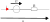
\includegraphics{c-3-1}
\subsection{Exemple}
On va transformer la partie encadrée en vert :

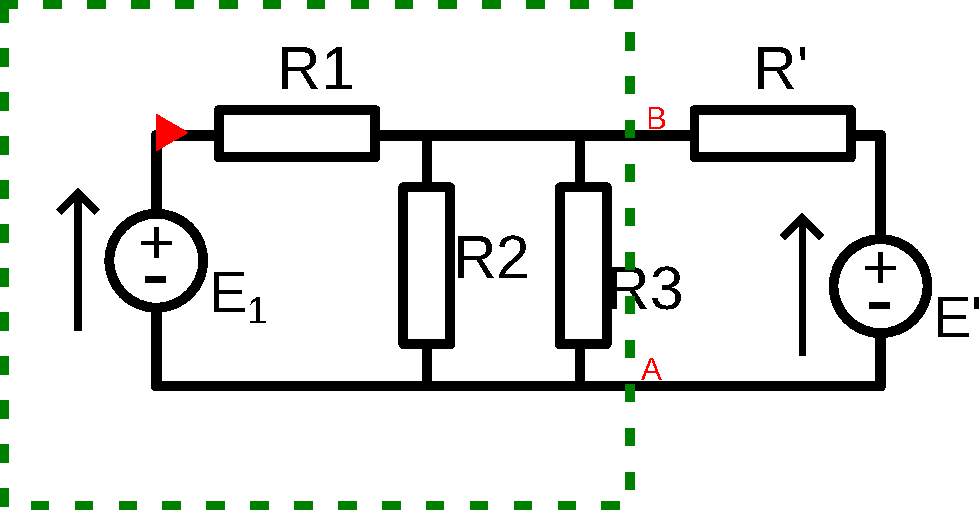
\includegraphics[scale=0.4]{c3-6}

Le but est de d'abord trouver $E_{th}$ en débranchant l'autre partie $\Delta$ du circuit.

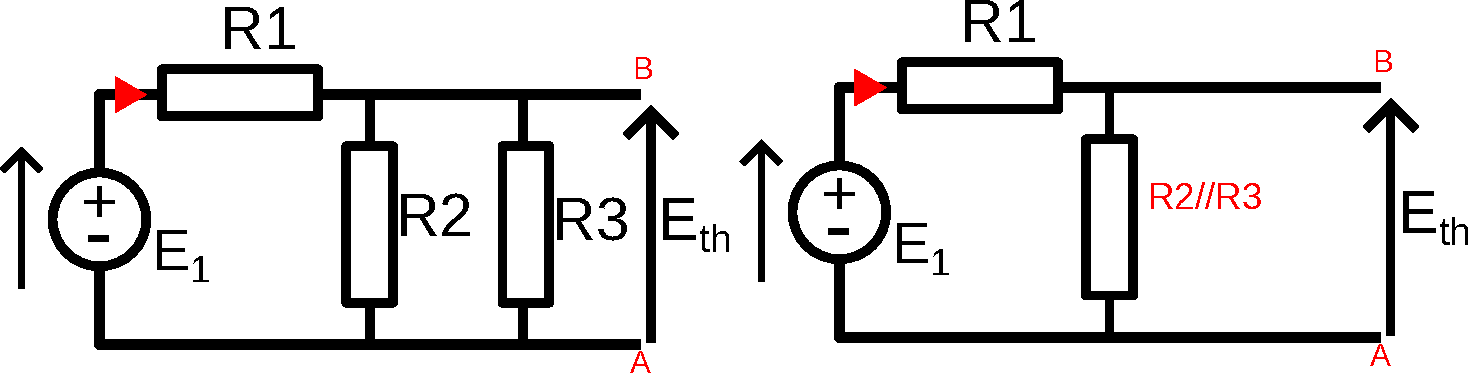
\includegraphics[scale=0.4]{c3-7}

On introduit une résistance équivalente et on remarque que $E_{th} = U_{r2//r3}$. En appliquant un pont diviseur de tension entre $R_1$ et la résistance équivalente, on trouve :

$E_{th} = U_{r2//r3} = E_1 \times \frac{R_2//R_3}{R_1+R_2//R_3} = E_1 \frac{R_2R_3}{R_1R_2+R_2R_3+R_1R_3}$

Pour trouver la résistance équivalente $R_{th}$, on passive les générateurs et on obtient 2 résistances en parallèle, soit $R_{th} = \frac{R_1\times R_2R_3}{R_1R_2+R_2R_3+R_1R_3}$

\section{Théorème de Norton}
On remplace une partie d'un circuit par un générateur de courant en parallèle d'une résistance. On se place dans les m\^emes hypothèses que Thévenin.
\begin{theorem}[Théorème de Norton]
 $D$ est modélisable par un générateur de courant de valeur $I_{N} = $ l'intensité du courant passant dans un court-circuit substitué à $\Delta$ associé à une résistance $R_{N}$ en parallèle égale à $R_{th}$
\end{theorem}
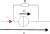
\includegraphics{c-3-2}
% Exemple : Pour trouver $I_N$, on replace $R_4$ par un court circuit. $I_N = i_1+i_2$ et $V_A-V_B = 0 \Rightarrow U_2-E_2 = 0 \Rightarrow R_2i_2 = E_2 \Rightarrow i_2 = \frac{E_2}{R_2}$. De la m\^eme façon, on obtient $i_1 = \frac{E_1}{R_1+R_3}$, donc $I_N = \frac{E_2}{R_2}+\frac{E_1}{R_1+R_3}$.
%
% Pour $R_N = R_2//(R_1+R_3) = \frac{R_2(R_1+R_3)}{R_1+R_2+R_3}$.

\warningInfo{équivalence}{On a $R_{th} = R_N$ et $E_{th} = R_{th} I_N$.}
\section{Théorème de Milmann}
\begin{theorem}
 Le potentiel en un point d'où partent $i$ branches contenant une résistance \(R_i\) et un générateur de tension \(U_i\)s'exprime comme : \[V_A = \frac{\sum_i \frac{U_i}{R_i}}{\sum_i G_i}\]
\end{theorem}

\end{document}

